\documentclass[11pt]{beamer}
\usepackage[utf8]{inputenc}
\usepackage[german]{babel}
\usepackage{amsmath}
\usepackage{graphicx}
\usetheme{default}
\setbeamertemplate{footline}[frame number]
\begin{document}
	\author{Gerald ..., Moritz ..., Tim Herbermann, Sebastian Siebert}
	\title{Akustik}
	\subtitle{eine Versuchsreihe}
	%\logo{}
	%\institute{}
	%\date{}
	%\subject{}
	%\setbeamercovered{transparent}
	\setbeamertemplate{navigation symbols}{}
	\frame[plain]{\maketitle}
	
	\begin{frame}
		\frametitle{Einleitung}
		Seite 1
	\end{frame}
	\begin{frame}
		\frametitle{Schall}
		Seite 2
	\end{frame}
	\begin{frame}
		\frametitle{Laufzeitmessung \qquad Veruschsaufbau}
		\begin{center}
			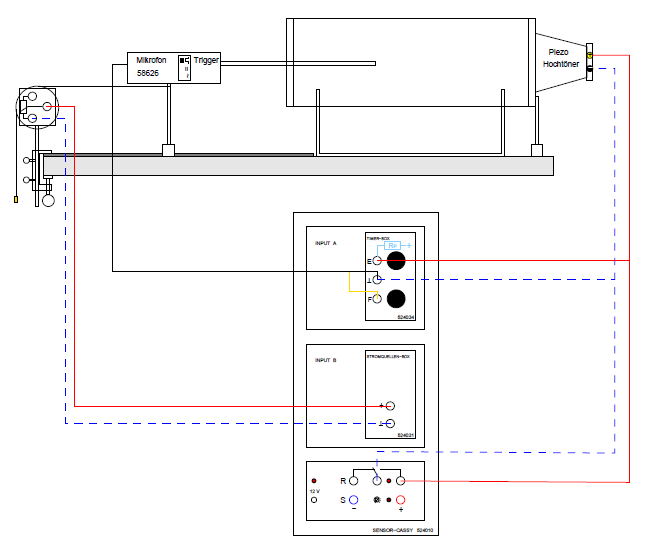
\includegraphics[width=0.8\linewidth]{aufbau_laufzeitmessung}
		\end{center}
	\end{frame}
	\begin{frame}
		\frametitle{Laufzeitmessung \qquad Rohdaten}
		\begin{center}
			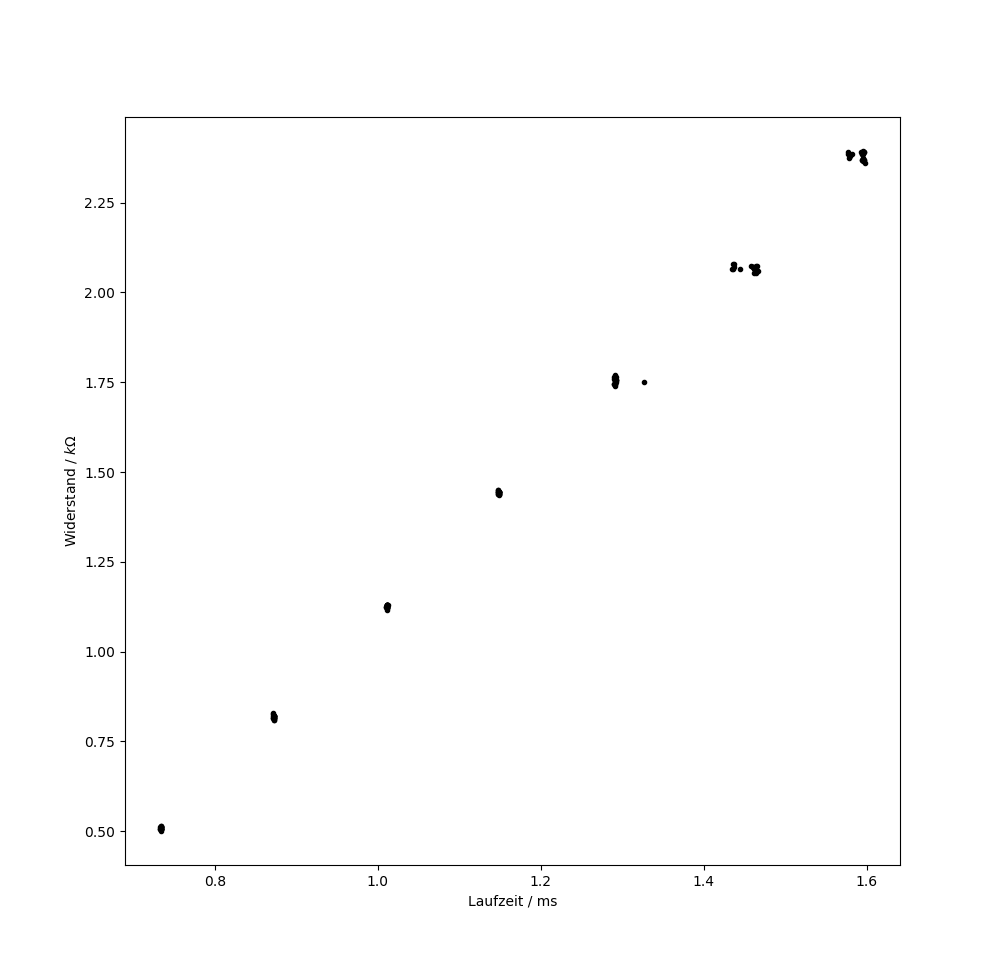
\includegraphics[width=0.8\linewidth]{rohdaten_laufzeit}
		\end{center}
	\end{frame}
	\begin{frame}
		\frametitle{Laufzeitmessung \qquad Auswertung}
		\begin{center}
			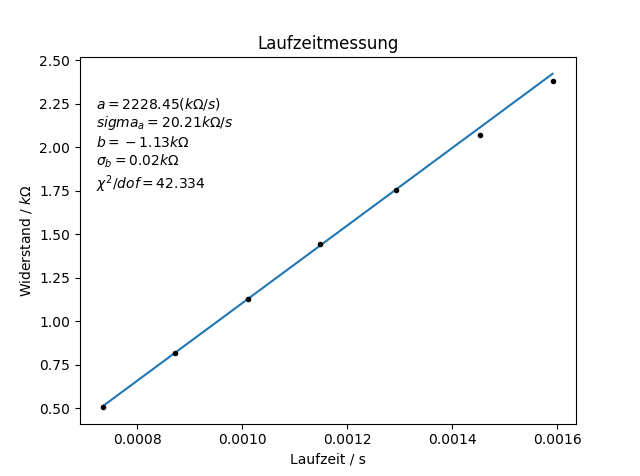
\includegraphics[width=0.6\linewidth]{fit_laufzeit}
		\end{center}
		$\bullet$ Kalibration Poti: $\frac{\Delta s}{\Delta R} = (15,99 \pm 0,07) \frac{cm}{k\Omega}$\\[0.4cm]
		$\bullet$ Laufzeitmessung: $\frac{\Delta R}{\Delta t} = (2181,55 \pm 22,77) \frac{k\Omega}{s}$\\[0.4cm]
		$\Rightarrow v = \frac{\Delta s}{\Delta t} = (348,90 \pm 3,64 \pm 1,53) \frac{m}{s}$
	\end{frame}
\end{document}